Recalling from the related work chapter \ref{ch:relatedwork}, DDPG is an off-policy algorithm that combines the \textit{Deterministic Policy Gradient} algorithm first introduced by \cite{silver2014deterministic} with the stability mechanisms of Deep Q-Learning (DQN). One major advantage of DDPG being a policy gradient method is the fact that it is able to handle problems with continuous action spaces  \cite[p.3]{lillicrap2019continuous} whereas DQN is limited to the discrete cases. This limitation arises due to the calculation of "best" actions given by the greedy policy $\max\limits_{a} Q(s_{t+1},a)$ which - for a discrete action space - is trivial. The Q-Learning algorithm just uses the expected return of the next state by simply selecting the one action in the set of actions that results in the highest consecutive Q-value. For the continuous case however, (Deep) Q-Learning would require an optimization of $a_t$ at every timestep to find the greedy policy which according to \cite{lillicrap2019continuous} "is too slow to be practical with large, unconstrained function approximators and nontrivial action spaces" (p.3).
\par
To overcome this challenge, policy gradient methods are conceptually different to action-value methods such as Q-Learning. Instead of learning action-values and using those estimates to derive a policy from, policy gradient methods maintain a function that can directly select actions without consulting a value function. This parameterized function $\mu_\theta(s)$ deterministically maps states to actions \cite[p.3]{lillicrap2019continuous} and represents the first component of the architecture - the \textit{actor}.
\par 
The actor adjusts the parameters $\theta$ of the policy in the direction of the performance gradient \cite[p.~2]{silver2014deterministic}. DDPG is an off-policy algorithm, which means that the ever-improving policy (target policy) is different from the one that interacts with the environment and gathers experience (behavior policy $\beta$). Therefore the off-policy deterministic policy gradient is defined and proven by \cite{silver2014deterministic} to be (p.~5): 
\begin{equation}
\begin{aligned}
    \nabla_{\theta^\mu}J &\approx \EX_{s_t \sim p^\beta}[
    \nabla_{\theta^\mu} Q(s,a\!\mid\! \theta^Q)\!\mid\! s\!=\!s_t, a\!=\!\mu(s_t\!\mid\!\theta^\mu)
    ] \\
    &= \EX_{s_t \sim p^\beta}[
    \nabla_a Q(s,a \!\mid\! \theta^Q) \!\mid\! s\!=\!s_t, a\!=\!\mu(s_t) \nabla_{\theta_\mu} \mu(s \!\mid\! \theta^\mu) \!\mid\! s\!=\!s_t]
    \end{aligned}
\end{equation}

\begin{equation}\label{eq:policyGradient}
    \nabla_\theta J_\beta (\mu_\theta) = 
    \EX_{s \sim p^\beta}
    \Big[ \nabla_\theta \mu_\theta(s) \; \nabla_a Q^\mu (s,a) \!\mid_{a = \mu_\theta (s)} \! \Big]
\end{equation}


As we can see in equation \ref{eq:policyGradient}, the performance gradient not only depends on gradient of the policy with respect to the policy parameters but also on the true action-values $Q^\mu(s,a)$ with respect to the actions for the current actor policy $\mu$. Since the true action-values are unknown, a differentiable function $Q^ \omega(s,a)$ replaces $Q^\mu(s,a)$ in order to estimate those values. This estimation is done off-policy from trajectories generated by $\beta(a\!\mid\!s)$ using an appropriate policy evaluation algorithm like Temporal-Difference-Learning or Q-Learning \cite[p.~5]{silver2014deterministic}. $Q^ \omega(s,a)$ is also called the \textit{critic} and represents the second component of the actor-critic architecture. The word "critic" is used because $Q^ \omega(s,a)$ evaluates the returns for the current behaviour of the actor and simultaneously improves his performance because the actor ascends the gradient of the critic.
\par
DDPG utilizes neuronal networks as non-linear function approximators for the actor and critic. As mentioned earlier, the usage of those powerful approximators require additional modifications as convergence is no longer guaranteed \cite[p.3]{lillicrap2019continuous}. Those modifications include the two introductions of a replay buffer and a specific exploration noise which are discussed in detail in the next two sub-chapters but also the employment of mini-batches, batch-normalization and most perceptibly target networks. The target networks are essentially copies of the actor and critic networks ($\mu'_\theta(s)$ and $Q'^\mu(s,a)$) and their initial weight distributions. After each update to the actor and critic networks, a "soft" update is performed as well, which adjusts the weights of the target networks to a very small extent in the direction of the learned networks.
\begin{figure}[H]
    \centering
    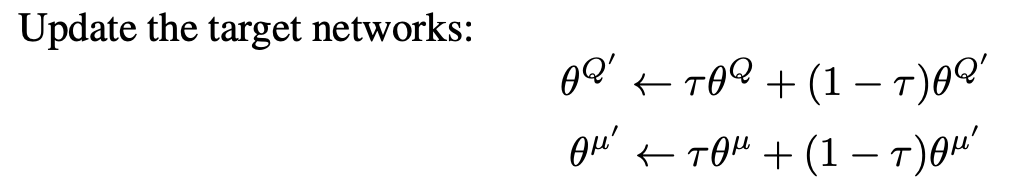
\includegraphics[width=0.75\textwidth]{images/ddpg_code/update_target.png}
    \caption{Illustration of the accumulated prediction error by bootstrapping input sequences for an LSTM}
    \label{fig:lstm}
\end{figure}
//TODO INSERT CODE BLOCK INSTEAD OF IMAGE \par

\cite{lillicrap2019continuous} explain that "the target values are constrained to change slowly, greatly improving the stability of learning" and "that having both a target $\mu'$ and $Q'$ was \textit{required} to have stable targets in order to consistently train the critic without divergence" (p.~4).